\section{Template Metaprogramming Approach}

\begin{figure}[htp]
\includegraphics[width=3.3in]{../overview}
\caption{template transformation}\label{fig:overview}
\end{figure}

\hspace{-1ex}\begin{figure}[htp]
\includegraphics[width=4.0in]{../mmexample}
\caption{Matrix-multiplication Example}\label{fig:mmexample}
\end{figure}

%programming model
Libvina utilizes C++ template mechanism to
perform source-to-source transformation for multicores. We uses
\emph{tasks} to abstract side-effect free functions. A task is
wrapped in the form of template class. \emph{TF classes} are able to
manipulate tasks, which take responsiblilty for transforming a tasks
into a group of subtasks. Finally, we map subtasks
into threads for specific architectures. Fig.~\ref{fig:overview}
depicts the diagram of template-based programming model.

\renewcommand\linenumberfont{\normalfont\small}
\setlength\linenumbersep{0.02in}
\linenumbers
\begin{verbatim}
template <class ARG0, class ARG1, 
          class RESULT,
  template <class, class> class PRED/*predicate*/
         int K,   /*param to divide task*/
        >
struct SGEMM {
 typedef view2_trait<ARG0> trait_arg0
 //omit other trait classes...

 typedef typename 
   ReadView2<typename trait_arg0::type,
                      trait_arg0::M / K,
                      trait_arg0::N / K>
 SubARG0;
 //omit other arguments definitions...


 typedef SGEMM<SubARG0, SubARG1, SubRESULT, 
               PRED, K> SubTask;

 typedef TF_hierarchy<SubTask, SubARG0, SubARG1,
                      SubRESULT, PRED>
 TF;

 static void //static entry
 doit(const ARG0& arg0, const ARG1& arg1, 
       RESULT& res)
 {
   //lambda for iteration
   auto subtask = [&](int i, int j) 
   {
      //temporaries
      Matrix<typename trait_res::type, 
             SubARG0::M, 
             SubARG1::N> tmp[K];

      //lambda for map
      auto m = [&](int k) {
        TF::doit(arg0.subR<SubARG0::M, SubARG0::N>(i, k), 
                 arg1.subR<SubARG1::M, SubARG1::N>(k, j),
                 tmp[k].subW());
      };
      //lambda for reduce
      auto r = [&](int i, int j) {
           tmp[i] += tmp[j];
      } 
      mapr<K, decltype(m)&, decltype(r)&>
      ::apply(m, r, res[i][j]);
   };
      
   typedef decltype(subtask)& closure_t;
   par< par<par_tail, K>, K, closure_t>
   ::apply(par_lv_handler2(subtask));  
 }/*end func*/f

 void 
 operator() (const ARG0& arg0, const ARG1& arg1, 
             RESULT& res)
 {
    //algorithm of matrix-multiplication
    //omit...
 }
};
\end{verbatim}
\nolinenumbers

\resetlinenumber[1]
\linenumbers
\begin{verbatim}
//template full specialization for langpipe
template<>
struct TF_pipeline<>
{
  //last stage defintions
  //T* is the type of input parameter.
  template<class T>
  static void impl(T* in)
  {
    //omit...
  }
 template<class T>
 static void doit(T * in)
 {
   std::tr1::function<void (T*)> 
     func(&(impl<T>));

   mt::thread_t thr(func, in);
 } 
};

//customize pipeline TF class
typedef TF_pipeline<
   translate<Eng2Frn>,
   translate<Frn2Spn>, 
   translate<Spn2Itn>,
   translate<Itn2Chn>
> MYPIPE;

MYPIPE::doit(&input);
\end{verbatim}
\nolinenumbers

Applications using our template-based programming model are free to
choose parallel pattern. An example using hierarchical division like
Sequoia is shown in Fig~\ref{fig:mmexample}. A matrix-multiplication application can be divided
into many submatrices multiplication and reduced them into the
result. We can apply a TF class dedicated to this parallel pattern and
it hierarchically generates a subtasks and reductions. The decomposition rule
and termination of recursion is programmed in template
metaprogramming.  

%meaning
Our programming model facilitates to separate two roles in software
development. Algorithm-centric programmers only concern of algorithm
in convential C/C++ form. They provide computation-intensive and
side-effect free functions in the form of task. On the other side,  system
programmers known underlying architecture are charge in developing and
applying template class to specialize tasks for the concrete
target. This separation not only solve the difficulties of writing and
tuning multicore, but also providing a uniform programming model to
develop effecient and portable parallel programs.

%discuss of stortcomes
The primary limitation of libvina is that we perform
transformation using template metaprorgramming.  Only static
information, \textit{i.e.} static constant value and types in C++, is
available at compile time. For example, we utilize array
dimensions(as template arguments) to estimate problem size in aforementined
matrix-multiplication programs. Thus, our programming model orients to
programs which contain rich static information. In embedded and
scientific applictions, the runtime with fixed parameters are
significantly longer than compile time even the time developing
programs. Therefore, metaprogramming will pay off 

%Another example depicted in ~\ref{fig:pipeexample}
%illustrates another parallel pattern in our programming model. It is
%psuedo langage translationg program using pipeline processing. Applying a TF class
%for 4 the taskscan synthesize a calling chain. 
\section{Libvina: A template library}
We implement a template library, libvina,  to demonstrate our approach. 
Libvina consists of 3 components: (1) Data structures, associated with
static information as template parameters. (2) Building blocks,
provides basic iterations to divide tasks (3) TF class, a TF class
represent a parallel pattern. 

\subsection{Data Structure}
To leverage static information, libvina need to
associate template parameters with ADTs' parameters. For example, for
Matrix class, it cantains 3 template paramters: type, the number of
row, the number of column.

A \emph{View} class is a concept to represent data set.
Fig. ~\ref{fig:view} depicts relationship of views in libvina. Concrete lines
represent implicit conversion in C++, while  dashed lines are explicit
function calls to complete conversion. Text in edges are constraints
when conversions perform. Shadow region is another thread space. The
only approach to communicate with other threads is through a special
kind of view called \emph{ViewMT}.  

The primary aim of view class is to hide communication. For shared
memory system or communication-exposed multcore \cite{cell, imagine}, 
we have chance to implement data movement according to target's archictures.
In addition, a view class is type-safed. Programmers can get
compilation errors if programs have potential violations of date
access rules. Early errors are particularly important to prevent programmer from trapping into multi-threaded bugs.

\begin{figure}
\includegraphics[width=3.3in]{../view_concept}
\caption{View classes in libvina}
\label{fig:view}
\end{figure}
%%
\subsection{Buiding Block}
Libvina provides a group of building blocks to execute
subtasks. To parallelize program, we expect that most subtasks are
executed in SPMD(Single-Program-Multiple-Thread). However, we needs to
deal with dependences carefully to guarantee correctness.  

Similar to constructs in traditional programming languages, our
building block support nesting defintion. Both \textit{seq} and
\textit{par} is interoperatable. for example, we can define a block as
follows:
\begin{verbatim}
seq<par<par_tail, 4>, 3, F>::apply();
\end{verbatim}
build to level-2 loop, and the nested loop are executed in
parallel. Its equivalence in OpenMP as follows:
\begin{verbatim}
int i, j;
F f;
for (i=0; i<3; ++i)
{
  #pragma omp parallel private(j)
  for (j=0; j<4; ++j) 
    f(i, j);
}
\end{verbatim}

\begin{table}[hbt]
\caption{Build blocks in libvina}
\begin{tabular}{|l|l|r|}
\hline
Name& Semantics& Example\\
\hline
\textbf{seq} & execute \textit{F} in squence & seq$<$seq\_tail, 5, F$>$::apply();\\
\hline
\textbf{par} & execute \textit{F} in paralllel & par$<$par\_tail, 4,
F$>$::apply();\\
\hline
\textbf{mapr}& execute \textit{M} in parallel, 
\textit{R}& mapr$<$8, F, R$>$::apply()\\
& and then perform after barrier&\\
\hline
\end{tabular}
\end{table}
\subsection{TF class}
TF class is the short form of \textit{TRansformation class}.  A
side-effect free function is referred to as
\emph{task} in libvina. Mathematically, a function is
single-target binary relation. As a rule of thumb,
computation-intensive functions are usually
self-contained, \textit{i.e.} external data references are limited and
calling graphs are simple. Therefore, it's possible to
decouple a task into a cluster of subtasks. The subtasks may be identical
except for arguments and we can distribute them on multicore to execute in
parallel.  Another approach is to divide a complicated task into finer stages
and run in pipeline manner to respect data locality and bandwidth. A
\textit{TF class} is a template class repsenting a parallel pattern which
transforms a task to a cluster of subtasks in
isomorphism.\textit{i.e.} the transformed task has the same interface
while owns a call graph to complete the original computation by a
cluster of subtasks. TF class also takes responsibility for
programming execution model.

To demonstrate more than one paralleling model, we implement two TF
class as follows:
\begin{itemize} 
\item TF\_hierarchy It will recursively generate subtasks until
  predicate is evaluate as true. As Fig.~\ref{mmexample} depict, We use
  TF\_hierarchy to implement programming model similar to Sequoia.

\item TF\_pipeline Input arbirary number of function, the template
  class can synthesize a call chain. This is common pattern for
  streaming programming mode.
\end{itemize} 

\section{User Adaption for Libvina}
User programmers need to customize their code to utilize
Libvina. Technically speaking, we provide a group of \emph{Concepts} to
support transformation and expect user
programmer \textit{Model} our template classes. 

\subsection{Function Wrapper}
Function wrapper is an idiom in libvina. Our approach needs to manipulate
template functions according to their template arguments.However, a
template function is unaddressable until it is instantiated. So user
programmers have to bind their template functions to static entries of
classes.  Line 25 of List.~\ref{lst:mm} is the case. In order to
cooperate with other entities, naming convention of entry is
predefined. In libvina, TF classes use name \textit{doit} and building
blocks use \textit{apply}. 

\subsection{Adaption for TF\_hierarchy}
Line.7~23 in Fig.~\ref{list:mm} are adaption for TF\_hierarchy. The
codes define the type of SubTask for SGEMM at Line.18. It is used to define
TF\_hierarchy class as TASK template parameter. PRED template
parameter at Line.22 is a predicate and TF\_hierarchy class will evaluate it using SubARG0 and
SubARG1. Line.39 calls customized TF class after dividing
task. According to template argument, TF class determine whether
reenter the static entry at Line. 25 or call \textit{call} operator at
Line.57 to perform computaton. Fig.~\ref{fig:hierarhcy} illustrates
instantiation process of TF\_hierarchy and the final result is
depicted in Fig.~\ref{mmexample}
\begin{figure}[hpt]
\includegraphics[width=3.5in]{../algo}
\caption{Algorithm of TF\_hierarchy}\label{fig:hierarchy}
\end{figure}
%for sequoia's programming mode: 
%define recursive rules 
% for stream 's programming model:
\subsection{Adaption for TF\_pipeline}
To leverage TF\_pipeline, user programmers have to provide a full
specialization template class for it. It is because that TF\_pipeline
can only synthesize functions and execute it in sequence. It does not
know how to process the output. A full specialization of TF\_pipeline very defines
this behavior and is called at last. For our example of
\textit{langpipe}, Line.2~20 is the case. static entry at Line.13 is
served for TF\_pipeline. We spawn a thread to handle with the output of
precious last stage. Line.23~28 is a usage of TF\_pipeline with 4
standalone functions. It is noteworthy that each function e.g
\textit{translate$<$Frn2Spn$>$} has to follow type interfaces and
define dependences. In \textit{lang\_pipe} case, we utilize our ViewMT
despicted in Fig.~\ref{fig:view}. ReadViewMT is only generated from
WriteView or WriteViewMT. The first case represents intialization. The
second builds dependence transparently when type conversion occurs.
We use signal mechanism to provoke downstreaming
stages. Fig.~\ref{fig.viewmt} illustrates the scenario contains 3
threads.

\begin{figure}[htp]
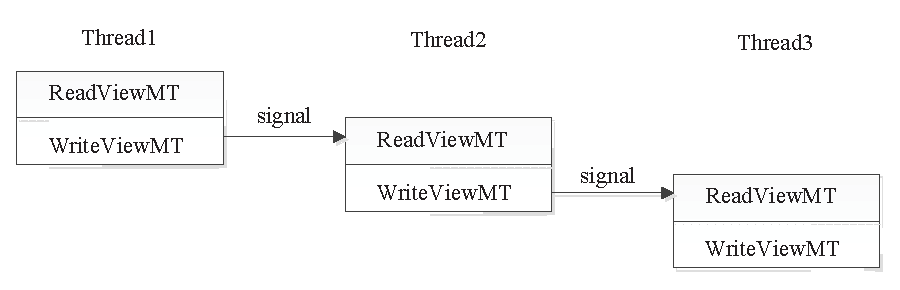
\includegraphics[width=3.1in]{../viewmt}
\caption{ViewMT in pipelining}\label{fig:viewmt}
\end{figure}

\section{Implementation details}
We implement all the functionalities described before using C++
template metaprogramming technique. The grand idea is to utilize
template specialization and recursion to achieve control flow at
compile time. Besides template mechanism, other  C++ high level
abstracts act important roles in our approach. Function object and bind
mechnism is critical to postpone computation at proper place with
proper enviroment~\cite{modernc++}. To utilize nested buiding blocks,
lambda expression generate closure object~\cite{cpplambda} at current
enviroment. 

\subsection{buiding block}
Implemenation of building blocks are trivial. We use recursive calls
to support nest. \textit{seq} and \textit{par} are interoperatable
because we chose proper nested class before calling.  It is worthy
noting that building blocks are level awareless. The function object
or cloure object need to be wrapped by loop-variable handlers. The
handlers take responsibility for calculating loop variable in
normalized form. It is only desirable for nest loop forms,
e.g. Line.53 in List.~\ref{lst::mm}.\textit{par}
embeds OpenMP directive to run in parallel on CPU. We don't implement
GPU counterpart because we can not see any benefits. 
\subsection{TF class}
\subsubsection{TF\_hierarchy}
We utilize predicate similar to merge~\cite{merge} to generate subtask
hierarchically. The major difference is that our predicate is
\textit{metafunction} and is evaluated at template parameter
declaration at place(Line.4).

\resetlinenumber[1]
\linenumbers
\begin{verbatim}
template <class TASK
  class ARG0, class ARG1, class RESULT,
  template<class, class>  class PRED,
  bool SENTINEL = PRED<ARG0, ARG1>::value>
struct TF_hierarchy{...}

template <class TASK
  class ARG0, class ARG1, class RESULT,
  template<class, class>  class PRED>
struct 
TF_hierarchy<TASK,ARG0,ARG1,RESULT,true>
{...};
\end{verbatim}
\nolinenumbers

\subsubsection{TF\_pipeline}
We implement the TF class using variadic template in C++0x. The
simplest implementation is listed as follows. It supports arbitrary
number of function, only limited by compiler's the maximal level of template
recursion.  For C++ compilers don't support variadic template, there
are workarounds to achieve the same effect, but quite tedious

\resetlinenumber[1]
\linenumbers
\begin{verbatim}
 template <class P, typename... Tail>
  struct pipeline<P, Tail...> {
    typedef typename P::input_type in_t;
    typedef typename P::output_type out_t;
   
    static out_t doit(in_t in)
    {
     pipeline<Tail...>::doit( P::doit(in) );
    }
  };  
\end{verbatim}
\nolinenumbers
